\section{Performance evaluation}
First of all we did an execution with the default parallel versions, the granularity set by default. With N=1000000000 and 8 threads, the worksharing constructs version lasts 10.84 seconds and the task version lasts 19 seconds. We see that there is a big difference between these two versions, this can be due to the overhead of creating and distributing the work during execution.

\subsection{Playing with worksharing constructs schedule}
\justify
All the tests have been done with N=1000000000. The following table summarises the tests done.

\begin{table}[!h]
\begin{tabular}{|l|l|}
\hline
Version               & Time (seconds) \\ \hline
schedule(auto)        & 10.7           \\ \hline
default               & 10.84          \\ \hline
schedule(static)      & 10.9           \\ \hline
schedule(static,1024) & 13.5           \\ \hline
schedule(static,256)  & 14             \\ \hline
schedule(static,1)    & 20             \\ \hline
schedule(dynamic, 1)  & -              \\ \hline
\end{tabular}
\end{table}
\justify
We conclude that is better to let the compiler decide. The better performance we obtain is when we let the compiler decide. Also point out that when we set scheduling to dynamic the computation does not end. Notice the similar time between \textit{schedule(auto)}, \textit{default} and \textit{schedule(static)} this may be due to the compiler generates similar code.
\subsection{Playing with taskloop grainsize num\_tasks}
All the tests have been done with N=1000000000 and 8 processors. The following table summarises the tests done.

\begin{table}[!h]
\begin{tabular}{|l|l|}
\hline
Version          & Time (seconds) \\ \hline
num\_tasks(4*nt) & 17             \\ \hline
num\_tasks(8*nt) & 17.4           \\ \hline
num\_tasks(nt)   & 19             \\ \hline
grainsize(8*nt)  & 68             \\ \hline
\end{tabular}
\end{table}
\justify
Notice that we got and improvement since the default version. The default version may be having load balancing problems that is solved with adding a finner grainsize, for example, 4 tasks for each thread which ensures all threads do the same work and we dont loose time with synchronisation, as it happens in the case grainsize(8*nt).  

\subsection{Strong scallability plots}
For a final performance evaluation, we get the strong scallability plots of the best performing versions of both approaches.
\justify
For the worksharing constructs version we obtain the following plot.

\begin{figure}[h!]
    \centering
    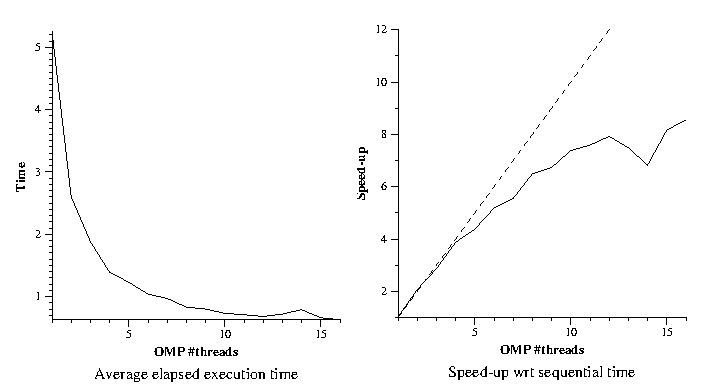
\includegraphics[width=0.9\textwidth]{strongFOR.png}
    \caption{Strong scallability plot for worksharing constructs approach}
\end{figure}

We can observe that the scallability stops being ideal from 5 threads, but is still scaling good from 5 threads. Let's now compare it to the task based plots.

\begin{figure}[h!]
    \centering
    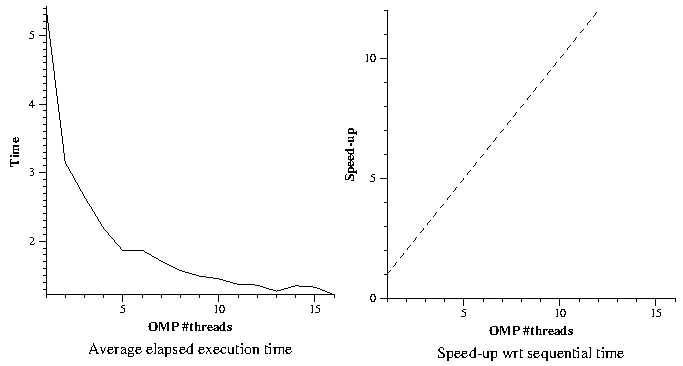
\includegraphics[width=0.9\textwidth]{strongTASK.png}
    \caption{Strong scallability plot for task based approach}
\end{figure}

It haven't been possible to get the plots due to the script is doing undefined behaviour. It's reporting 0 of speedup, that obviously, it's not the correct speedup.

\subsection{Time comparison}
Also to compare execution times more clearly I executed both versions with N=100000000 and 1, 2, 4, 8, 12 processors.


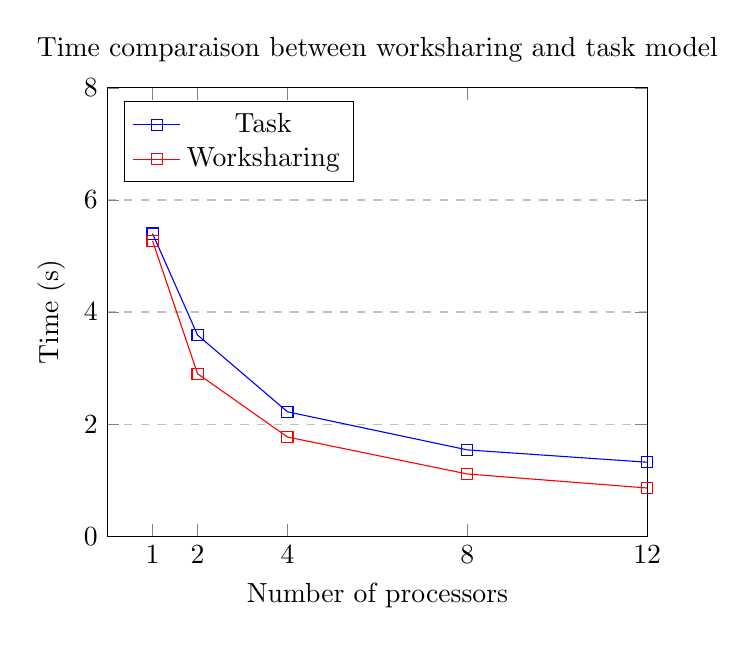
\begin{tikzpicture}
\begin{axis}[
    title={Time comparaison between worksharing and task model},
    xlabel={Number of processors},
    ylabel={Time (s)},
    xmin=0, xmax=12,
    ymin=0, ymax=8,
    xtick={1,2,4,8,12},
    ytick={0,2,4,6,8},
    legend pos=north west,
    ymajorgrids=true,
    grid style=dashed,
]
 
\addplot[
    color=blue,
    mark=square,
    ]
    coordinates {
    (1,5.4)(2,3.59)(4,2.22)(8,1.54)(12,1.32)
    };
    \addlegendentry{Task}
 
 \addplot[
    color=red,
    mark=square,
    ]
    coordinates {
    (1,5.27)(2,2.9)(4,1.77)(8,1.11)(12,0.86)
    };
    \addlegendentry{Worksharing}
\end{axis}
\end{tikzpicture}

\justify
We can observe that the difference is small but worksharing constructs version performs better. Also point out that the scalability is really similar.







